% document formatting 
\documentclass[10pt]{article}
\usepackage[utf8]{inputenc}
\usepackage[left=1in,right=1in,top=1in,bottom=1in]{geometry}
\usepackage[T1]{fontenc}
\usepackage{xcolor}

% math symbols, etc.
\usepackage{amsmath, amsfonts, amssymb, amsthm}
\usepackage{dsfont}

% lists
\usepackage{enumerate}
\usepackage{tabularx}
\usepackage{multirow}
\usepackage{array}
\usepackage{blkarray}

% images
\usepackage{graphicx} % for images
\usepackage{tikz}
\usetikzlibrary{matrix}

% code blocks
\usepackage{minted, listings} 

% verbatim greek
\usepackage{alphabeta}
\DeclareMathOperator*{\argmin}{arg\,min}
\DeclareMathOperator*{\argmax}{arg\,max}
\newcommand{\dd}{\text{d}}

\graphicspath{{./assets/images/}}

\title{02-620 Week 11 \\ \large{Machine Learning for Scientists}}
 
\author{Aidan Jan}

\date{\today}

\begin{document}
\maketitle

\section*{Hidden Markov Models (HMMs)}
For example: speech processing.
\begin{itemize}
	\item Observations: sound signals
	\item Hidden states: parts of speech, words, etc.
\end{itemize}

\subsection*{The First Use of HMMs in Biology}
\textbf{Finding Genes:} The first draft of a human genome sequence (2001):
\begin{center}
\texttt{cggtgaaactgcacgattgttgctggcttaaagatagaccaatcagagtgtgtaacgtct
atttagcgtcttctatcatccaatcactgcactttacacactataaatagagcagctcag
tgggcgtatttgcgctagtgttgggtgttccgctgtgctgtttttccgtcatggctcgca
tcctaagcaaactgctcggaagtctactggtggcaaggcgccacgcaaacagttggccac
aggcagcccgcaaaagcgctccggccaccggcggcgtgaaaaagccccaccgctacccgg
gcaccgtggctctgcgcgagatccgccgttatcagaagtccactgaactgcttattcgta
aactacctttccagcgcctggtgcgcgagattgcgcaggactttaaaacagacctgcgtt
tccagagctccgctgtgatggctctgcaggaggcgtgcgaggcctacttggtagggctat
ttgaggacactaacctgtgcgccatccacgccaagcgcgtcactatcatgcccaaggaca
tccagctcgcccgccgcatccgcggagagagggcgtgattactgtggtctctctgacggt
ccaagcaaaggctcttttcagagccaccaccttttcaagtaaagtagctgtaagaaacca
atttaagacaaaagggaatgcattgggagcacttttcgttttaatgctactgaaggc}
\end{center}
Where are the genes? 
\begin{itemize}
	\item In this case, the observations are the nucleotides
	\item The hidden states are introns, exons, and intergenic regions
\end{itemize}
Researchers David Haussler and Jim Kent used HMMs to search for which base pairs were more likely to be genes:\\\\
\begin{center}
\texttt{\textcolor{blue}{cggtgaaactgcacgattgttgctggcttaaagatagaccaatcagagtgtgtaacgtct
atttagcgtcttctatcatccaatcactgcactttacacactataaatagagcagctcag
tgggcgtatttgcgctagtgttgggtgttc}\textcolor{red}{cgctgtgctgtttttccgtcatggctcgca
tcctaagcaaactgctcggaagtctactggtggcaaggcgccacgcaaacagttggccac
aggcagcccgcaaaa}\textcolor{green}{gcgctccggcca}\textcolor{red}{ccggcggcgtgaaaaagccccaccgctacccgg
gcaccgtggctctgcgcgagatccgccgt}\textcolor{green}{tatcagaagtccactgaactgcttattcgta
aactacctttccagcgcctggtgcgcgagattgcgcagg}\textcolor{red}{actttaaaacagacctgcgtt
tccagagctccgctgtgatggctctgcaggaggcgtgcgaggcctacttggtagggc}\textcolor{blue}{tat
ttgaggacactaacctgtgcgccatccacgccaagcgcgtcactatcatgcccaaggaca
tccagctcgcccgccgcatccgcggagagagggcgtgattactgtggtctctctgacggt
ccaagcaaaggctcttttcagagccaccaccttttcaagtaaagtagctgtaagaaacca
atttaagacaaaagggaatgcattgggagcacttttcgttttaatgctactgaaggc}}
\end{center}
\begin{itemize}
	\item Blue: intergenic regions
	\item Green: Introns
	\item Red: Exons
\end{itemize}

\subsection*{Overview}
A Hidden Markov Model (HMM) is used to model a set of observations with a set of hidden states.
\begin{itemize}
	\item Hidden states generate observations
	\item Hidden states transition to other hidden states
\end{itemize}

\subsection*{Hidden Markov Model as Bayesian Network}
\begin{itemize}
	\item The joint probability if $(Q, O)$ is defined as
\end{itemize}
\begin{center} 
	\includegraphics*[width=0.6\textwidth]{W10_6.png} 
\end{center}
\begin{itemize}
	\item The $q_i$'s are ``states''.  These are random variables that take values from a set $S = \{s_1, \dots, s_n\}$, e.g., $\{I, E, B\}$ in the gene example.
	\item The $o_i$'s are ``outputs''.  These are random variables that take values from a set $\Sigma = \{\sigma_1, \dots, \sigma_m\}$, e.g., $\{A, C, T, G\}$ in the gene example.
\end{itemize}

\subsection*{HMM definition: Conditional Probability}
\begin{itemize}
	\item We just defined random variables.  How do we define the conditional probability distributions for each random variable?
	\begin{itemize}
	    \item Initial state probability
	    \item Transition probability
	    \item Emission probability
    \end{itemize}
\end{itemize}

\subsubsection*{Conditional Probability Parents}
$q_1$:
\begin{itemize}
	\item $P(q_1 = s_i) = \pi_i$, with $\Pi = \{\pi_1, \dots, \pi_n\}$
	\item The probability that we \textit{start} at state $s_i$, $i = 1, \dots, n$
	\item Called ``initial state probability''
\end{itemize}
$q_2, \dots, q_T$:
\begin{itemize}
	\item $P(q_t = s_i | q_{t - 1} = s_j)$
	\item Defined as a $n \times n$ matrix
	\item Called a ``transition probability''
\end{itemize}
\[P(q_2 | q_1) = P(q_3 | q_2) = \dots = P(q_T | q_{T - 1})\]
$o_1, \dots, o_T$:
\begin{itemize}
	\item $P(o_t = \sigma_j | q_t = s_i)$
	\item Defined as a $n \times m$ matrix for $n$ states and $m$ output values
	\item Called ``emission probability''
\end{itemize}
The \textbf{joint probability} of ($Q = \{q_1, \dots, q_T\}, O = \{o_1, \dots, o_T\}$) is defined as
\[P(Q, O) = P(q_1) P(o_1 | q_1) \prod_{t = 2}^T P(q_t | q_{t - 1}) P(o_t | q_t)\]
\begin{itemize}
	\item $Q$ represents the hidden states, and $O$ represent the observed states
    \item The first term ($P(q_1)$) is the initial state probability
	\item The second term and the last term ($P(o_1 | q_1)$ and $P(o_t | q_t)$) are emission probabilities
	\item $P(q_t | q_{t - 1})$ are transition probabilities
\end{itemize}

\subsection*{HMM Summary}
Random variables:
\begin{itemize}
	\item States (latent): $q_1, \cdots, q_T$
	\item Outputs (observed): $o_1, \cdots, o_T$
\end{itemize}
Probability distribution
\begin{itemize}
	\item Initial state probability: $P(q_1 = s_i)$
	\item Transition probability: $P(q_t = s_i | q_{t - 1} = s_j)$
	\item Emission probability: $P(o_t = \sigma_j | q_t = s_i)$
\end{itemize}

\subsection*{HMM Example: Rolling one of 2 dice}
\begin{itemize}
	\item A sequence of dice rolls
	\item For each time, choose from two dice A and B, each with 6 faces
	\item Current die depends on the previous die
\end{itemize}
\begin{center}
\begin{tabular}{|c|c|c|c|c|c|c|c|c|c|c|c|}
    \hline
    \textbf{Hidden states:} & A & A & A & B & B & B & B & B & B & A & A \\ \hline
    \textbf{Observations:} & 1 & 6 & 2 & 1 & 4 & 2 & 1 & 1 & 1 & 2 & 5 \\ \hline
\end{tabular}
\end{center}
\begin{center}
\begin{tabular}{ll|lll|llll}
\cline{3-5} \cline{7-9}
\multicolumn{1}{c}{} & \multicolumn{1}{l|}{~\hspace{1.5cm}~} & \multicolumn{3}{c|}{Emission Probability} & \multicolumn{1}{l|}{~\hspace{1.5cm}~} & \multicolumn{3}{c|}{Transition Probability} \\ \cline{3-5} \cline{7-9} 
 &  & \multicolumn{1}{l|}{$v$} & \multicolumn{1}{l|}{$P(v | A)$} & $P(v | B)$ & \multicolumn{1}{l|}{} & \multicolumn{1}{l|}{$t \setminus t + 1$} & \multicolumn{1}{l|}{$A$} & \multicolumn{1}{l|}{$B$} \\ \cline{3-5} \cline{7-9} 
Initial State Probability: &  & \multicolumn{1}{l|}{1} & \multicolumn{1}{l|}{0.3} & 0.1 & \multicolumn{1}{l|}{} & \multicolumn{1}{l|}{$A$} & \multicolumn{1}{l|}{0.8} & \multicolumn{1}{l|}{0.2} \\ \cline{3-5} \cline{7-9} 
\multirow{2}{*}{$\begin{cases} \Pi_A = 0.7 \\ \Pi_b = 0.3 \end{cases}$} &  & \multicolumn{1}{l|}{2} & \multicolumn{1}{l|}{0.2} & 0.1 & \multicolumn{1}{l|}{} & \multicolumn{1}{l|}{$B$} & \multicolumn{1}{l|}{0.2} & \multicolumn{1}{l|}{0.8} \\ \cline{3-5} \cline{7-9} 
 &  & \multicolumn{1}{l|}{3} & \multicolumn{1}{l|}{0.2} & 0.1 &  &  &  &  \\ \cline{3-5}
 &  & \multicolumn{1}{l|}{4} & \multicolumn{1}{l|}{0.1} & 0.2 &  &  &  &  \\ \cline{3-5}
 &  & \multicolumn{1}{l|}{5} & \multicolumn{1}{l|}{0.1} & 0.2 &  &  &  &  \\ \cline{3-5}
 &  & \multicolumn{1}{l|}{6} & \multicolumn{1}{l|}{0.1} & 0.3 &  &  &  &  \\ \cline{3-5}
\end{tabular}\\
\vspace{2em}
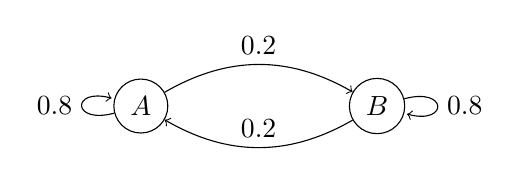
\begin{tikzpicture}
    \node[draw, circle] at (0, 0) (0) {$A$};
    \node[draw, circle] at (3, 0) (1) {$B$};

    \draw[->] (0) edge[bend left=30] node [above] {0.2} (1);
    \draw[->] (1) edge[bend left=30] node [above] {0.2} (0);
    \draw[->] (0) edge[loop left] node [left] {0.8} (0);
    \draw[->] (1) edge[loop right] node [right] {0.8} (1);
\end{tikzpicture}
\end{center}

\subsection*{HMM Inference: Forward-Backward}
\begin{itemize}
	\item Can you infer ``unobserved'' from ``observed''?  $P(Q | O)$
	\item In the DNA example, we would have $q_t: \{\text{Exon, Intron, Background}\}$, $o_t: \{A, T, C, G\}$
	\item What is the probability of candidate intron/exon/intergenic region labels given the nucleotide sequence?
\end{itemize}
The Forward-Backward Algorithm is the following:
\begin{itemize}
	\item Compute forward variables
	\item Compute backward variables
	\item Given results of the above, perform inference
	\begin{itemize}
	    \item $P(Q | O)$ for a sequence of states $Q = \{q_1, \dots, q_T\}$, given observations $O = \{o_1, \dots, o_T\}$
	    \item $P(q_t = s_i | O)$, given observations $O = \{o_1, \dots, o_T\}$
	    \item Find the most probable path (of states) $\argmax_Q P(Q | O)$
    \end{itemize}
\end{itemize}

\subsection*{The Forward Algorithm}
\begin{itemize}
	\item Goal: $\alpha_t(i) = P(o_1, \cdots, o_t, q_t = s_i)$, for $t = 1, \cdots, T$ and $s_i = 1, \cdots, n$
	\item Initialization: $\alpha_1(i) = P(o_1, q_1 = s_i)$, by definition.  We can write this as $P(o_1 | q_1 = s_i) P(q_1 = s_i)$.
	\begin{itemize}
	    \item The first probability is the emission probability, and the second is the initial state.
    \end{itemize}
	\item Forward recursion: update $\alpha_{t + 1}(i)$ given $\alpha_t(j), j = 1, \cdots, n$.
	\[\alpha_{t + 1}(i) = \sum_{j = 1}^n P(o_{t + 1} | q_{t + 1} = s_i) P(q_{t + 1} = s_i | q_t = s_j) \alpha_t(j)\]
    This can be simplified to
    \[\sum_{j = 1}^n P(o_{t + 1} | q_{t + 1} = s_i) P(q_{t + 1} = s_i | q_t = s_j) \alpha_t(j)\]
    \begin{itemize}
	    \item The first probability in the sum is emission probability.  The second is transition probability.
    \end{itemize}
\end{itemize}

\subsection*{The Backward Algorithm}
\begin{itemize}
	\item Goal: $\beta_t(i) = P(o_{t + 1}, \cdots, o_T | q_t = s_i)$, for $t = 1, \cdots, T$ and $s_i = 1, \cdots, n$
	\item Initialization: $\beta_T(i) = P(o_{T + 1} | q_T = s_i) = 1$
	\item Backward recursion: update $\beta_t(i)$ given $\beta_{t + 1}(j)$, $j = 1, \cdots, n$.
	\[\beta_t(i) = \sum_{j = 1}^n P(q_{t + 1} = s_j | q_t = s_i) P(o_{t + 1} | q_{t + 1} = s_j) \beta_{t + 1}(j)\]
    This can be simplified to
    \[\sum_{j = 1}^n \beta_{t + 1}(j) P(o_{t + 1} | q_{t + 1} = s_j) P(q_{t + 1} = s_j | q_t = s_i)\]
    \begin{itemize}
	    \item The beta term is recursion, the first probability in the sum is the transition probability, and the second is the emission probability.
    \end{itemize}
\end{itemize}

\subsection*{HMM: Inference}
\begin{itemize}
	\item Given the results of the forward-backward algorithm, perform inference
	\begin{itemize}
	    \item $P(Q | O)$ for a sequence of states $Q = \{q_1, \dots, q_T\}$, given observations $O = \{o_1, \dots, o_T\}$
	    \item $P(q_t = s_i | O)$, given observations $O = \{o_1, \dots, o_T\}$
	    \item Find the most probable path (of states) $\argmax_Q P(Q | O)$
    \end{itemize}
\end{itemize}
What is $P(Q | O)$, for a sequence of states $Q = \{q_1, \dots, q_T\}$ given observations $O = \{o_1, \dots, o_T\}$?
\begin{itemize}
	\item We can use Bayes rule!  We know that $P(O | Q) = P(o_1 | q_1) P(o_2 | q_2) \dots P(o_T | q_T)$
	\item We also know $P(Q) = P(q_1) P(q_2 | q_1) \dots P(q_T | q_{T - 1})$
	\item But how do we find $P(O)$?  $P(O) = P(o_1, \dots, o_T) = \sum_i P(o_1, \dots, o_T, q_T = s_i) = \sum_i \alpha_T (i)$
	\begin{itemize}
	    \item For $n$ states and a sequence of length $T$, finding $P(O)$ takes $O(n^2 T)$ time!  The others are linear in $T$ ($O(T)$)
    \end{itemize}
\end{itemize}
Can we find $P(q_t = s_i | O)$, given observations $O - \{o_1, \dots, o_T\}$?
\begin{itemize}
	\item Using Bayes rule, we have
	\begin{align*}
    P(q_t = A | o_1, \dots, o_T) &= \frac{P(o_1, \dots, o_t, o_{t + 1}, \dots, o_T, q_T = A)}{P(o_1, \dots, o_T)} \\
    &= \frac{P(o_1, \dots, o_t, q_t = A) P(o_{t + 1}, \dots, o_T | q_t = A)}{P(o_1, \dots, o_T)} \\
    &= \frac{\alpha_t(A) \beta_t (A)}{\sum_i \alpha_t(i) \beta_t(i)}
    \end{align*}
    \item We can in fact solve for $P(q_t = s_i | O)$ using the forwards and backwards results!
\end{itemize}
To find the most probable path, we solve $\argmax_Q P(Q | O)$.
\begin{itemize}
	\item This can be rewritten using Bayes rule to be $\frac{P(O | Q) P(Q)}{P(O)}$, which we can drop the $P(O)$ since it does not depend on $Q$.
	\item We do this using the \textbf{Viterbi algorithm}
\end{itemize}

\subsection*{The Viterbi Algorithm}
\begin{itemize}
	\item $\delta_t(i)$: maximum probability of ending up at state $s_i$ at observation $t$ (out of all possible sequences of states leading up to it)
	\item Initialization: $\delta_1(i) = P(o_1 | q_1 = s_i) P(q_1 = s_i)$
	\item Update: $\delta_{t + 1}(i) = \max_j P(o_{t + 1} | q_{t + 1} = s_i) P(q_{t + 1} = s_i | q_t = s_j) \delta_t(j)$
\end{itemize}
Once we have $\delta_T(i)$, we can solve for our $P(Q^* | O)$ by:
\[P(Q^* | O) = \max_Q P(Q | O)\]
Where $Q^* = \argmax_Q P(Q | O)$, or the path defined by $\argmax_j \delta_t(j)$
\begin{itemize}
	\item Goal: find most probable path $Q = [q_1, \cdots, q_T]$ given observation $O = [o_1, \cdots, o_T]$
	\item $\delta_t(i) = \max_{q_1, \cdots, q_t} P(q_1, \cdots, q_t | o_1, \cdots, o_t)$
	\item Solve by iteration:
	\begin{itemize}
	    \item $\delta_1(i) = P(o_1 | q_1 = s_i) P(q_1 = s_i)$
	    \item $\delta_{t + 1}(i) = \max_j P(o_{t + 1} | q_{t + 1} = s_i) P(q_{t + 1} = s_i | q_t = s_j) \delta_t(j)$
    \end{itemize}
\end{itemize}

\section*{Learning HMMs}
The graph structure is always ``known'' or ``fixed''.  Learning the parameters, or the conditional probability distributions:
\begin{itemize}
	\item The hidden variables are observed: MLE
	\item The hidden variables are unobserved: EM
\end{itemize}

\subsection*{Learning when Hidden States are Observed}
\begin{itemize}
	\item Assume both hidden and observed variables are observed
	\item Data: $((O^1, Q^1), \dots, (O^k, Q^k))$ for $K$ sequences, where $O^k = (o_1^k, \dots, o_T^k)$, $Q^k = (q_1^k, \dots, q_T^k)$
\end{itemize}
MLE for learning:
\begin{align*}
&\argmax \log p((O^1, Q^1), \dots, (O^k, Q^k)) = \prod_k P(O^k, Q^k) \\
&= \argmax sum_k \log p(q_1^k) + \sum_k \log p(o_1^k | q_1^k) + \sum_k \sum_t \log p(o_t^k | q_t^k) + \sum_k \sum_t \log p(q_t^k | q_{t - 1}^k)
\end{align*}
\begin{itemize}
	\item Note that the first sum only involves initial probabilities, the second and third terms only involve emission probabilities, and the last term only involves transition probabilities
	\item Differentiate with respect to each of the parameters and set it to 0 to solve!
	\item Closed-form solution.
\end{itemize}
However, in most cases, we do not know what states generated each of the outputs (states are unobserved/hidden)
\begin{itemize}
	\item but had we known, it would be very easy to determine an emission and transition model with MLE!
	\item On the other hand, if we had such a model we could determine the set of states using the inference methods from before
\end{itemize}

\subsection*{Expectation Maximization (EM)}
\begin{itemize}
	\item Appropriate for problems with `missing values' for the variables.
	\item For example, in HMMs we usually do not observe the hidden variables (the states)
	\item Assume complete data log likelihood and maximize \textbf{expected log likelihood}
	\begin{align*}
        &\argmax E[\log p((O^1, Q^1), \dots, (O^k, Q^k))] \\
        &= \argmax E\left[\log \prod_k \left[p(q_1^k) p(o_1^k | q_1^k) \prod_{t = 2}^T p(q_t^k | q_{t - 1}^k) p(o_t^k | q_t^k)\right]\right]
    \end{align*}
    where the expectation is taken with respect to $p(Q | O, \text{ parameters})$
\end{itemize}

\subsubsection*{Aside: EM Steps}
There are two steps:
\begin{itemize}
	\item E step: Fill in the missing variables with the expected values
	\item M step: Regular maximum likelihood estimation (MLE) using the values computed in the E step and the values of the other variables
\end{itemize}
This is guaranteed to converge, though only to a local minima.

\subsection*{E-Step}
In our example, with complete data, we needed ``actual counts''
\begin{itemize}
	\item \#A, \#B to estimate initial probabilities and emission probabilities
	\item \#AA, \#AB, \#BA, \#BB to estimate transition probabilities
\end{itemize}
When hidden states are not observed, we need ``expected counts'' in the E step.

\subsubsection*{State and Transition Probabilities}
\begin{itemize}
	\item Probability of a state given observations: (definition)
	\[P(q_t = s_i | o_1, \dots, o_T) = \frac{\alpha_t(i) \beta_t(i)}{\sum_j \alpha_t(j) \beta_t(j)} = S_t(i)\]
    \item We can also derive a transition probability given observations: (definition)
    \begin{align*}
    &P(q_t = s_i, q_{t + 1} = s_j | o_1, \cdots, o_T) \\
    &= \frac{\alpha_t(i) P(q_{t + 1} = s_j | q_t = s_i) P(o_{t + 1} | q_{t + 1} = s_j) \beta_{t + 1}(j)}{\sum_j \alpha_t(j) \beta_t(j)} = S_t(i, j)
    \end{align*}
\end{itemize}

\rule{\textwidth}{2pt}

First, we want to compute $S_t(i)$ and $S_t(i, j)$ for all $t$, $i$, and $j$ ($1 \leq t \leq T, 1 \leq i \leq k, 1 \leq j \leq k$) 
\begin{align*}
    &P(q_t = s_i | o_1, \dots, o_T) = S_t(i) \\
    &P(q_t = s_i, q_{t + 1} = s_j | o_1, \dots, o_T) = S_t(i, j)
\end{align*}

\subsection*{M-Step}
Compute transition probabilities, $a_{i, j} = p(q_t = s_j | q_{t - 1} = s_i)$
\[a_{i, j} = \frac{\hat{n}(i, j)}{\sum_k \hat{n}(i, k)}\]
where
\[\hat{n}(i, j) = \sum_t S_t(i, j)\]

Now, we compute emission probabilities (assume a multinomial distribution):  Let
\[B_k(j) = \sum_{t | o_t = j} S_t(k)\]
then \textbf{the emission probability} $b_k(j) = P(o_t = j | s_i = k)$
\[b_k(j) = \frac{B_k(j)}{\sum_i B_k(i)}\]

\subsection*{Summary EM-Algorithm}
The EM algorithm for learning parameters of HMMs is the \textbf{Baum-Welch} algorithm.\\\\
Inputs: Observations $O_1, \dots, O_T$, $S = $ number of states in HMM
\begin{enumerate}
	\item Guess initial transition and emission parameters
	\item Compute \textbf{E-step}: $S_t(i)$ and $S_t(i, j)$
	\item Compute \textbf{M-step}
	\item Convergence?  (If not, go to step 2)
	\item Output complete model.
\end{enumerate}

\subsection*{States in HMM}
How to decide on the number of states in HMM?
\begin{itemize}
	\item More states means a more complex model, overfitting!
\end{itemize}
Model selection problem
\begin{itemize}
	\item Cross validation
	\item Nonparametric Bayesian model
\end{itemize}

\section*{Other Forms of Bayesian Networks}
\subsection*{Dynamic Bayesian Networks (DBNs)}
\begin{itemize}
	\item Bayesian networks for modeling dynamic process.  HMM is a special case of DBN.
	\begin{itemize}
	    \item HMM represents the state with \textbf{a single random variable}: $P(Q_t | Q_{t - 1})$
	    \item DBN represents the state with \textbf{a set of random variables}: $P(Q_t | Q_{t - 1})$, where $Q_t$ is a set of variables
    \end{itemize}
\end{itemize}

\subsection*{Factorial HMMs}
A Factorial HMM is a DBN with $D$ chains, each with $K$ states.
\begin{center} 
	\includegraphics*[width=0.5\textwidth]{W11_1.png} 
\end{center}

\subsection*{Other Variants of HMMs as DBNs}
\begin{center} 
	\includegraphics*[width=0.8\textwidth]{W11_2.png} 
\end{center}

\subsection*{Semi-Markov HMM}
\begin{itemize}
	\item Relax the Markov constraint to allow staying in the current state for an explicit duration of time $L_t$
\end{itemize}
\begin{center} 
	\includegraphics*[width=0.6\textwidth]{W11_3.png} 
\end{center}
\[P(Y_{t - l + 1:l} | Q_t, L_t = l) = \prod_{i = 1}^l P(Y_i | Q_t)\]

\subsection*{Hierarchical HMM}
\begin{itemize}
	\item Each state can emit another HMM that generates sequences
\end{itemize}
\begin{center} 
	\includegraphics*[width=0.5\textwidth]{W11_4.png} 
\end{center}

\subsection*{Practical Uses of HMMs}
In biology, it can be used to 
\begin{itemize}
	\item find DNA Motifs bound by transcription factor.
	\item sequence alignment (single and multiple species)
	\item Phylo-HMM (phylogenetics)
\end{itemize}

\subsection*{Summary: Important Points}
\begin{itemize}
	\item Why HMMs?
	\item Inference in HMMs
	\begin{itemize}
	    \item Forward-backward algorithm
	    \item Various inference tasks
	    \item Viterbi algorithm
    \end{itemize}
	\item Learning in HMMs
	\begin{itemize}
	    \item EM algorithm with inference as a subroutine
    \end{itemize}
\end{itemize}

\section*{Bayesian Learning}
\subsection*{General Strategies for Learning a Probability Model}
\begin{itemize}
	\item Maximum Likelihood Estimation (MLE)
	\begin{itemize}
	    \item Frequentist approach ($\theta$ is deterministic)
	    \item $\hat{\theta}_{MLE} = \argmax_\theta \log P(data | \theta)$
    \end{itemize}
    \item Maximum \textit{a posteriori} estimation (MAP):
    \begin{itemize}
	    \item Bayesian approach ($\theta$ is random)
	    \item $\hat{\theta}_{MAP} = \argmax_\theta \log P(\theta | data)$
    \end{itemize}
    \item Fully Bayesian appraoch
    \begin{itemize}
	    \item Estimate $P(\theta | data)$ (full distribution, not point estimate)
	    \item Close-form solution, direct sampling.  Gibbs sampling, etc.
    \end{itemize}
\end{itemize}

\subsubsection*{Example: Bayesian Inference for Linear Regression}
Model: $y = Xw + e$
\begin{itemize}
	\item Input: $X \in \mathbb{R}^{n \times m}$; output $y \in \mathbb{R}^n$
	\item Parameters: $w \in \mathbb{R}^m \sim N(0, \sigma_w^2)$ (IID)
	\item Noise: $e \in \mathbb{R}^n \sim N(0, \sigma_e^2)$ (IID)
\end{itemize}
Posterior distribution:
\[P(w | y, X) \propto P(y | X, w) P(w)\]
\begin{itemize}
	\item $P(y | X, w) = N(Xw, \sigma_e^2)$
	\item $P(w) = N(0, \sigma_w^2)$
\end{itemize}
MAP estimate:
\[\hat{w}_{MAP} = \left(X^T X + \frac{\sigma_e^2}{\sigma_w^2} I\right)^{-1} X^T y\]
\begin{itemize}
	\item Small $\sigma_0^2$ value means strong prior belief
\end{itemize}
Fully Bayesian estimation: full distribution vs. point estimate
\[P(w | y, X) = \frac{P(y | w, X) P(w)}{P(y | X)}\]

\subsubsection*{Point Estimate vs. Full Distribution}
\begin{itemize}
	\item MAP and MLE returns a point, $w^*$ that maximizes $P(w | Data)$.
	\item Fully Bayesian returns a full distribution of $P(w | Data)$
\end{itemize}

\subsubsection*{Fully Bayesian Linear Regression}
\begin{itemize}
	\item How can we learn the posterior $p(w | y, X)$?
	\begin{itemize}
	    \item Both likelihood and prior are Gaussian
	    \item By conjugacy, the posterior is also Gaussian
	    \[p(w | y, X) \sim N(\mu, \Sigma)\]
    \end{itemize}
    where
    \begin{itemize}
	    \item $\mu = \left(\frac{X^T X}{\sigma_e^2} + \frac{I}{\sigma_w^2}\right)^{-1} \left(\frac{X^T y}{\sigma_e^2}\right)$
	    \item $\Sigma = \left(\frac{X^T X}{\sigma_e^2} + \frac{I}{\sigma_w^2}\right)^{-1}$
    \end{itemize}
\end{itemize}

\subsection*{General Bayesian Inference}
Steps:
\begin{enumerate}
	\item Set up the probability model (e.g., mixture models, HMMs, linear regression, Bayesian networks, logistic regression, etc.)
	\item Determine the prior
	\item Determine the posterior distributions, based on Steps (1) and (2)
\end{enumerate}

\subsubsection*{Step 3: Easy case with Closed-Form Solutions}
\begin{itemize}
	\item How can you describe $p(w | Data)$
	\begin{itemize}
	    \item Parametric distribution for simple model (e.g., Gaussian)
	    \item Conjugacy
	    \begin{itemize}
	        \item Gaussian likelihood + Gaussian prior $\rightarrow$ Gaussian posterior
	        \item Binomial likelihood + Beta prior $\rightarrow$ Beta posterior
        \end{itemize}
    \end{itemize}
\end{itemize}

\subsubsection*{Step 3: Difficult case with Numerical Solutions}
\begin{itemize}
	\item How can you describe $p(w | Data)$
	\begin{itemize}
	    \item The exact form of the posterior distribution cannot be obtained for more complex models
	    \item Describe the posterior with a histogram of samples from $p(w | Data)$
    \end{itemize}
\end{itemize}

\subsection*{Posterior Inference for Linear Regression: Sampling as an Alternative Solution}
\begin{itemize}
	\item How can we learn the posterior $p(w | y, X)$?
	\begin{itemize}
	    \item How can we learn the posterior $p(w | y, X)$?
	    \begin{itemize}
	        \item Both likelihood and prior are Gaussian
	        \item By conjugacy, the posterior is also Gaussian
        \end{itemize}
        \item Draw samples from this posterior $p(w | y, X) \sim N(\mu, \Sigma)$
        \begin{itemize}
	        \item Draw 100 samples $w^1, \cdots, w^{100}$ from $p(w | y, X) \sim N(\mu, \Sigma)$
        \end{itemize}
        \item Compute any statistics of interest from the samples.
    \end{itemize}
\end{itemize}

\subsection*{General Numerical Approach: Sample from the Posterior Distribution}
Direct sampling
\begin{itemize}
	\item Draw 100 samples from $P(w | y, X)$
	\item For $i = 1, \dots, 100$:
	\begin{itemize}
    	\item Draw $w^i$ from $P(w | y, X)$
    	\item This yields $w^i = [w_1^i, \cdots, w_m^i]$
    \end{itemize}
\end{itemize}
When to use it:
\begin{itemize}
	\item Posterior doesn't have a closed-form solution, but we can sample from it.
\end{itemize}
What if:
\begin{itemize}
	\item We cannot sample from the joint distribution $P(w | Data)$,
	\item but we can \textbf{sample from the conditional distribution} $P(w_j | w_{-j}, Data)$ for each coordinate?  ($w_{-j}$ represents all elements of $w$ except $w_j$)
\end{itemize}

\section*{Gibbs Sampling}
Compare to direct sampling, Gibbs sampling:\\\\
Draw 100 samples from $P(w | y, X)$.  To do this:
\begin{itemize}
	\item Initialize $w^0$ with random values
	\item For $i = 1, \dots, 100$,
	\begin{itemize}
	    \item For $j = 1, \dots, m$,
	    \begin{itemize}
	        \item sample $w_j^i$ from $p(w_j | w_{1:j - 1}^i, w_{j + 1:m}^{i - 1}, Data)$
	        where $w_{1:j-1}^i$ is the $1$ to $(j-1)$-th elements of $w^i$, and $w_{j + 1:J}^{i - 1}$ is the $(j + 1)$ to $m$-th elements of $w^{i - 1}$.
        \end{itemize}
    \end{itemize}
\end{itemize}
The difference compared to direct sampling is that here, we are sampling from the \textbf{marginal distribution}, which is way easier than sampling from the joint distribution as in direct sampling.
\begin{itemize}
	\item If you run Gibbs sampling for many iterations, the samples from later iterations will approximate smaples from the target distribution, as if it were drawn from direct sampling
\end{itemize}
To draw a single sample $w^i$ in a single iteration,
\[P(w_1, w_2, w_3, w_4, \cdots, w_m | y, X)\]
\begin{itemize}
	\item $w_1$ is sampled from $P(w_1 | w_{2:m}^{i - 1}, y, X)$
	\item $w_2$ is sampled from $P(w_2 | w_1^i, w_{3:m}^{i - 1}, y, X)$
    \item $w_3$ is sampled from $P(w_3 | w_{1:2}^i, w_{4:m}^{i - 1}, y, X)$
    \item $w_4$ is sampled from $P(w_4 | w_{1:3}^i, w_{5:m}^{i - 1}, y, X)$
    \item \dots
    \item $w_m$ is sampled from $P(w_m | w_{1:m - 1}^i, y, X)$
\end{itemize}

\subsection*{Properties of Gibbs Sampling}
Initial samples are bad.  But when the iteration stabilizes:
\begin{itemize}
	\item The samples approximate the joint distribution of all variables.
	\item The marginal distribution of any subset of variables can be approximated by simply considering the samples for that subset of variables, ignoring the rest.
	\item The expected value of any variable can be approximated by averaging over all the samples.
\end{itemize}
We often discard the initial (burn-in) samples and keep the ones that are equivalent to drawing from $p(w | y, X)$

\subsection*{How Many ``Initial'' Iterations?}
How many burn-in iterations?
\begin{itemize}
	\item Too few iterations?
	\item Too many iterations?
	\item (we wait until the distribution stabilizes, and discard samples from before that point)
\end{itemize}
How many samples should we draw?
\begin{itemize}
	\item Too few iterations?
	\item Too many iterations?
	\item (We wait until the estimates stabilize.)
\end{itemize}

\section*{Markov Chain Monte Carlo (MCMC)}
\begin{itemize}
	\item In general, in more complex models, direct sampling from posterior distribution is not possible. 
	\item However, sampling from \textbf{a conditional posterior}, a distribution for a single variable conditional on all other variables, may be possible.  Gibbs sampling!
	\item For even more complex models, sampling from this conditional distribution is not possible.  Then, other \textbf{Markov chain Monte Carlo (MCMC)} methods!
	\begin{itemize}
	    \item Approximate the conditional posterior with a tractable distribution (Gaussian, uniform) to draw samples.
    \end{itemize}
\end{itemize}
One example of a different MCMC sampling is Metropolis-Hastings sampling (sampling multiple dimensions at once)

\subsection*{Gibbs Sampling and MCMC in Biology}
\begin{itemize}
	\item Gibbs sampling or MCMC is widely used for Bayesian learning / inference
	\begin{itemize}
	    \item Hidden Markov models: genome phasing
	    \item Mixture models: clustering genes, individuals, tumors
	    \item Probabilistic graphical models for discovering population structure (admixture model)
    \end{itemize}
\end{itemize}

\subsection*{Summary}
\begin{itemize}
	\item Bayesian Learning:
	\begin{itemize}
	    \item Fully Bayesian approach to learn the posterior distribution
	    \item Gibbs sampling as a special case of MCMC
    \end{itemize}
\end{itemize}


\end{document}